\documentclass[12pt,fleqn]{article}\usepackage{../../common}
\begin{document}
Materyel Mekaniği - 11

Üç boyutta herhangi bir yönde olabilecek bir kiriş öğesinin direngenlik
matrisini bu bölümde geliştirelim [2, sf. 281]. Literatürde bu yapılara uzay
çerçeveleri (space frame) denebiliyor. Bunu yapabilmek için daha önce gördüğümüz
eksenel, iki boyutlu kiriş, burulma direngenlik matrislerini birleştireceğiz.

İki boyuttaki kirişin mekaniği bükülme alttaki gibiydi [1],

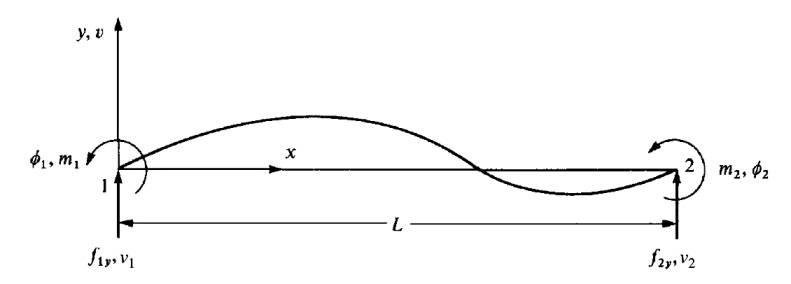
\includegraphics[width=25em]{phy_020_strs_11_02.jpg}

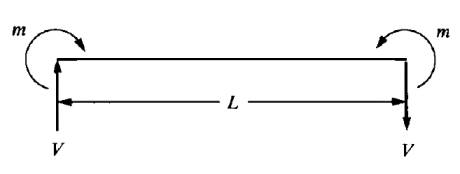
\includegraphics[width=25em]{phy_020_strs_11_03.jpg}

Şimdi işaretler alttaki gibi olacak,

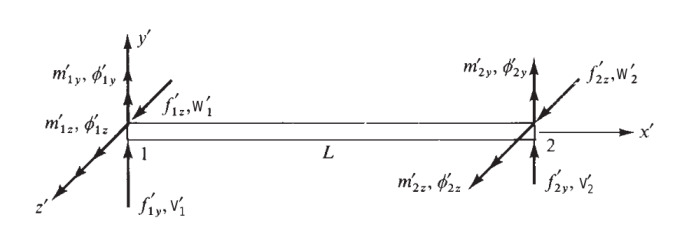
\includegraphics[width=25em]{phy_020_strs_11_01.jpg}

İki boyutlu kiriş matrisini [1] iki kez kullanacağız, ilki $x-z$ düzlemi icin,
ikincisi $x-y$ düzlemi için,

$x-z$ düzlemi

$$
\frac{EI_y}{L^4}
\left[\begin{array}{cccc}
12L & -6L  & -12L & -6L^2 \\
    & 4L^3 & 6L^2 & 2L^3  \\
    &      & 12L  & 6L^2  \\
    &      &      & 4L^3
\end{array}\right]
\mlabel{1}
$$

$x-y$ düzlemi

$$
\frac{EI_y}{L^4}
\left[\begin{array}{cccc}
12L & 6L  & -12L & 6L^2 \\
    & 4L^3 & -6L^2 & 2L^3  \\
    &      & 12L  & -6L^2  \\
    &      &      & 4L^3
\end{array}\right]
\mlabel{2}
$$

Dikkat edersek $x-y$ düzleminin matrisi [1] matrisi ile aynı. $x-z$ düzlemi
matrisinin bazı işaretleri farklı, bunun sebebi düzlemdeki bükülmenin sağ el
kuralına göre farklı yönleri gösterebilmesi. Mesela [1]'deki 

$$
m_1 = -m = -EI \frac{\ud^2 v(0)}{\ud x^2} =
\frac{EI}{L^3} ( 6L v_1 + 4L^2 \phi_1 - 6L v_2 + 2 L^2 \phi_2 )
$$

formülünü hatırlarsak, o formülde bir uçta $m$ diğer üçta $-m$ vardı, fakat
üstteki figürde $x-z$ düzlemindeki iki uçtaki $m$ değerleri aynı işarettedir,
sağ el kuralını düşünürsek $x-z$'deki bükülme 1 noktasında kağıttan bize doğru
gösteriyor, 2 noktasında aynı şekilde. O zaman üstteki formüldeki işaretler
değişir,

$$
\Rightarrow \frac{EI}{L^3} ( -6L v_1 - 4L^2 \phi_1 + 6L v_2 - 2 L^2 \phi_2 )
$$

Bir değişim daha açılarda, üstteki formülde $\phi_1,\phi_2$ olan acılar,
üç boyuttaki üstteki şekilde bunlar $\phi_{1y}$ ve $\phi_{2y}$. Bu açılar
iki boyutlu durumun aksine artı yönde tam ters işaretli, tersi yönde bir
yer değişim $v_1,v_2$'ye sebep oluyorlarlar, bu yüzden o işaretler de
tersine dönüyor, notasyonu da düzeltince,

$$
\Rightarrow \frac{EI}{L^3} ( -6L v_1 + 4L^2 \phi_{1y} + 6L v_2 + 2 L^2 \phi_{2y} )
$$

Böylece matrisin ikinci satırında $-6,+4,+6,+2$ katsayılarını elde ediyoruz.
Bu işaretlerin (1) matrisinin ikinci satırıyla aynı olduğunu görebiliriz,
diğer satırlar benzer şekilde değiştiriliyorlar.

Üstdüşüm (Superposition)

Artık bahsedilen matrisleri birleştirebiliriz. Bu üstdüşümü \verb!sympy!  ile
otomatik olarak yapacağız, daha önce sayısal değerler için kullandığımız
\verb!expand_dataframe! kodu yine kullanılabilecek, çünkü kod bir \verb!pandas!
Dataframe'i baz alıyor, bu Dataframe içinde herhangi bir obje depolamak mümkün,
oraya sayılar yerine \verb!sympy! sembolik matematik objeleri koyabiliriz. Bir
bonus ta elde ediyoruz, toplama işlemi \verb!sympy! tipleri için önceden
tanımlıdır, yani eğer üstdüşüm sırasında çakışma olursa, sembolik objeler
birbiriyle toplanacaktır!

\begin{minted}[fontsize=\footnotesize]{python}
from sympy import symbols, pprint, latex
from sympy.matrices import Matrix
import pandas as pd, pickle
pd.set_option('display.max_columns', None)

all_vars = ['u1','v1','w1','phi1x','phi1y','phi1z',\
            'u2','v2','w2','phi2x','phi2y','phi2z']
A,G,J,E,L,Iy,Iz = symbols("A,G,J,E,L,Iy,Iz")
\end{minted}

Önce üstte bahsedilen iki düzlemi alalım,

\begin{minted}[fontsize=\footnotesize]{python}
# x-z
vars1 = ['w1','phi1y','w2','phi2y']
M1 = pd.DataFrame([[12*L, -6*L**2,-12*L,-6*L**2],
                  [-6*L**2,4*L**3,6*L**2,2*L**3],
                  [-12*L,6*L**2,12*L,6*L**2],
                  [-6*L**2,2*L**3,6*L**2,4*L**3]],index=vars1)
M1.columns = vars1
M1 = M1 * (E*Iy/L**4 )
# x-y
vars2 = ['v1','phi1z','v2','phi2z']
M2 = pd.DataFrame([[12*L, 6*L**2,-12*L,6*L**2],
                  [6*L**2,4*L**3,-6*L**2,2*L**3],
                  [-12*L,-6*L**2,12*L,-6*L**2],
                  [6*L**2,2*L**3,-6*L**2,4*L**3]],index=vars2)
M2.columns = vars2
M2 = M2 * (E*Iz/L**4 )
\end{minted}

Şimdi [1]'deki eksenel yükleri tanımlayan makaskiriş direngenlik matrisini
alalım,

\begin{minted}[fontsize=\footnotesize]{python}
# Eksenel Yuk
vars3 = ['u1','u2']
M3 = pd.DataFrame([[1,-1],[-1,1]],index=vars3)
M3.columns = vars3
M3 = M3 * (A*E/L)
\end{minted}

[4]'te tanımladığımız burulma mekaniğinin matrisini belirtelim,

\begin{minted}[fontsize=\footnotesize]{python}
# Burulma (Torsion)
vars4 = ['phi1x','phi2x']
M4 = pd.DataFrame([[1,-1],[-1,1]],index=vars3)
M4.columns = vars4
M4 = M4 * (G*J/L)
\end{minted}

Hepsini üstdüşüm ile birleştirelim,

\begin{minted}[fontsize=\footnotesize]{python}
import sys; sys.path.append('../phy_020_strs_08')
import dfutil

M1f = dfutil.expand_dataframe(M1,all_vars)
M2f = dfutil.expand_dataframe(M2,all_vars)
M3f = dfutil.expand_dataframe(M3,all_vars)
M4f = dfutil.expand_dataframe(M4,all_vars)
Mall = Matrix(M1f + M2f + M3f + M4f)
pickle.dump(Mall,open("Mall.pkl","wb"))
\end{minted}

Sonuç matrisini bir dosyaya yazalım, 

\begin{minted}[fontsize=\footnotesize]{python}
print (latex(Mall)[:100],'...')
\end{minted}

\begin{verbatim}
\left[\begin{array}{cccccccccccc}\frac{A E}{L} & 0 & 0 & 0 & 0 & 0 & - \frac{A E}{L} & 0 ...
\end{verbatim}

$$
\left[\begin{array}{cccccccccccc}\frac{A E}{L} & 0 & 0 & 0 & 0 & 0 & - \frac{A E}{L} & 0 & 0 & 0 & 0 & 0\\0 & \frac{12 E Iz}{L^{3}} & 0 & 0 & 0 & \frac{6 E Iz}{L^{2}} & 0 & - \frac{12 E Iz}{L^{3}} & 0 & 0 & 0 & \frac{6 E Iz}{L^{2}}\\0 & 0 & \frac{12 E Iy}{L^{3}} & 0 & - \frac{6 E Iy}{L^{2}} & 0 & 0 & 0 & - \frac{12 E Iy}{L^{3}} & 0 & - \frac{6 E Iy}{L^{2}} & 0\\0 & 0 & 0 & \frac{G J}{L} & 0 & 0 & 0 & 0 & 0 & - \frac{G J}{L} & 0 & 0\\0 & 0 & - \frac{6 E Iy}{L^{2}} & 0 & \frac{4 E Iy}{L} & 0 & 0 & 0 & \frac{6 E Iy}{L^{2}} & 0 & \frac{2 E Iy}{L} & 0\\0 & \frac{6 E Iz}{L^{2}} & 0 & 0 & 0 & \frac{4 E Iz}{L} & 0 & - \frac{6 E Iz}{L^{2}} & 0 & 0 & 0 & \frac{2 E Iz}{L}\\- \frac{A E}{L} & 0 & 0 & 0 & 0 & 0 & \frac{A E}{L} & 0 & 0 & 0 & 0 & 0\\0 & - \frac{12 E Iz}{L^{3}} & 0 & 0 & 0 & - \frac{6 E Iz}{L^{2}} & 0 & \frac{12 E Iz}{L^{3}} & 0 & 0 & 0 & - \frac{6 E Iz}{L^{2}}\\0 & 0 & - \frac{12 E Iy}{L^{3}} & 0 & \frac{6 E Iy}{L^{2}} & 0 & 0 & 0 & \frac{12 E Iy}{L^{3}} & 0 & \frac{6 E Iy}{L^{2}} & 0\\0 & 0 & 0 & - \frac{G J}{L} & 0 & 0 & 0 & 0 & 0 & \frac{G J}{L} & 0 & 0\\0 & 0 & - \frac{6 E Iy}{L^{2}} & 0 & \frac{2 E Iy}{L} & 0 & 0 & 0 & \frac{6 E Iy}{L^{2}} & 0 & \frac{4 E Iy}{L} & 0\\0 & \frac{6 E Iz}{L^{2}} & 0 & 0 & 0 & \frac{2 E Iz}{L} & 0 & - \frac{6 E Iz}{L^{2}} & 0 & 0 & 0 & \frac{4 E Iz}{L}\end{array}\right]
$$

Bu matrisin [2, sf. 282]'deki matris ile aynı olduğunu göreceğiz.

Döndürme işlemine geldik, döndürme için bir $T$ matrisi gerekiyor ki daha önce
olduğu gibi bir $T^T k' T$ işlemini yapabilelim. Bu $T$ matrisi içinde dört tane
3x3 boyutunda $\lambda$ matris bloğu olacak, $T$ köşegeni üzerinde
tekrarlanacaklar, ki böylece her değişken bloğu çarpılabilsin /
döndürülebilsin. Bu bloklar $(u_1,v_1,w_1)$, $(\phi_{1x},\phi_{1y},\phi_{1z})$,
$(u_2,v_2,w_2)$, $(\phi_{2x},\phi_{2y},\phi_{2z})$ [2, sf. 282].

$$
T = \left[\begin{array}{cccc}
[\lambda] &  & & \\
 & [\lambda] & & \\
 & & [\lambda] & \\
 & & & [\lambda]
\end{array}\right]
$$

Her $\lambda$ matrisi ``yön kosinüsleri'' denen değerleri içeriyor olacak, bu
kavramın detayları için bkz [6, sf. 73], [5, sf. 224], özet olarak tarif etmek
gerekirse bir vektörün ya da yeni kordinat sisteminin yeni ekseninin, referans
bir diğer ekseni ile olan açısının kosinüsü olarak görebiliriz.

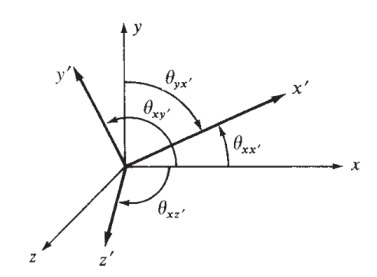
\includegraphics[width=20em]{phy_020_strs_11_04.jpg}

Eğer eksen değişimi, transformasyonunu hesaplıyorsak $y$ ekseninin yeni $x'$
ekseni ile oluşturduğu açı $\cos_{yx'}$ olarak gösterilebilir, ya da kısaca
$C_{yx'}$, tüm bu kombinasyonlar için elde edilen açılar bir matris içinde
$\lambda$'da yer alır,

$$
\lambda = \left[\begin{array}{ccc}
C_{xx'} & C_{yx'} & C_{zx'} \\
C_{xy'} & C_{yy'} & C_{zy'} \\
C_{xz'} & C_{yz'} & C_{zz'} 
\end{array}\right]
$$

Sonlu Öğeler (Finite Element) bu hesap şu şekilde uygulanır, FEM problemlerinde
genellikle yapılan bir kiriş parçası transform edilmiş $x'$ ekseni kabul edilir,
ve geri kalan $\lambda$ değerleri buna göre doldurulur. Bu durumda kirişin uç ve
baş noktasını kullanarak $x'$ ile oluşan açıları şöyle bulabiliriz,

$$
\cos_{xx'} = \frac{x_2 - x_1}{L} = l
$$

$$
\cos_{yx'} = \frac{y_2 - y_1}{L} = m
$$

$$
\cos_{zx'} = \frac{z_2 - z_1}{L} = n
$$

ki kirişin son noktası $x_2,y_2,z_2$, baş noktası $x_1,y_1,z_1$, uzunluk $L$.

Kiriş bazlı yeni eksen oluştururken bir kez $x'$ elde ettikten sonra diğer
eksenleri ona göre bulabiliriz, diğer herhangi bir vektörle oluşturulan düzleme
dik olan yeni bir vektörü $y'$ için kullanabilirdik mesela, [2]'de yapılan $x'$
ile $z$ ekseninin çapraz çarpımını almaktır. Bilindiği gibi iki vektöre dikgen
üçüncü bir vektör çapraz çarpım ile hesaplanır, böylece $x'$ eksenine dikgen bir
$y'$ elde etmiş oluruz, sonra $x'$ ile $y'$ ekseninin bir çapraz çarpımı daha
alınarak her iki eksene dikgen üçüncü eksen $z'$ bulunabilir.  Bu hesapla elde
edilen $x',y',z'$ bir kordinat ekseninin sahip olması gerekli tüm koşulları
yerine getiriyor.

Biraz önceki semboller üzerinde görelim, $i,j,k$ birim vektörler, notasyonda
genellikle $\mathbf{i},\mathbf{j},\mathbf{k}$ olarak gösterilirler.

$$
z \times x' = y' = \frac{1}{D}
\left[\begin{array}{ccc}
i & j & k \\ 0 & 0 & 1 \\ l & m & n
\end{array}\right]
$$

$$
y' = - \frac{m}{D} i + \frac{l}{D} j
$$

$$
D = (l^2 + m^2)^{1/2}
$$

Simdi $z'$ ekseni,

$$
z' = x' \times y' = \frac{1}{D}
\left[\begin{array}{ccc}
i & j & k \\ l & m & n \\ -m & l & 0
\end{array}\right]
$$

$$
z' = -\frac{ln}{D} i - \frac{mn}{D} j + D k 
$$

Sonuçları bir araya koyarsak,

$$
\renewcommand*{\arraystretch}{2.0}
\lambda = \left[\begin{array}{ccc}
l & m & n \\
-\dfrac{m}{D} & \dfrac{l}{D} & 0 \\
-\dfrac{ln}{D} & -\dfrac{mn}{D} & D
\end{array}\right]
$$

Üstteki matris bir vektörü yerel kordinat sisteminden global kordinat sistemine
çevirebilir. $T$ içinde üstteki matrisleri kullanırız, ve $T^T k' T$ hesabını
yaparız.

Problem 5.7

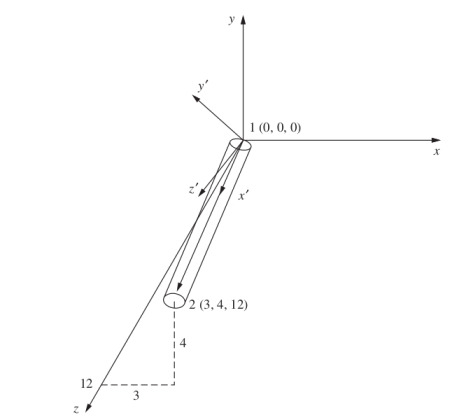
\includegraphics[width=20em]{phy_020_strs_11_05.jpg}

Üstteki şekil için gereken $\lambda$ matrisini bulun [2, sf. 285].

Çözüm

Önce kiriş uzunluğunu bulalım.

\begin{minted}[fontsize=\footnotesize]{python}
np.sqrt(3**2 + 4**2 + 12**2)
\end{minted}

\begin{verbatim}
Out[1]: 13.0
\end{verbatim}

Şimdi uzunluğu kullanarak $x'$ eksenini bulalım, daha önce bahsedildiği gibi bu
eksenin çubuğun bir ucundan başlayıp onunla aynı yönü gösterdiği kabul edilir.
Bu değerlere $l_x,l_y,l_z$ diyelim, $\lambda$ matrisinin ilk satırı bu değerler,

$$
l_x = \frac{x_2 - x_1}{L} = \frac{3 = 0}{13} = \frac{3}{13}
$$

$$
m_x = \frac{y_2 - y_1}{L} = \frac{4-0}{13} = \frac{4}{13}
$$

$$
n_x = \frac{z_2 - z_1}{L} = \frac{12 = 0}{13} = \frac{12}{13}
$$

Şimdi $D$ hesabını yapabiliriz,

$$
D = (l_x^2 + m_x^2)^{1/2} =
\left[
  \left(\frac{3}{13}\right)^2 +
  \left(\frac{4}{13}\right)^2
\right]^{1/2} = \frac{5}{13}
$$

$y'$ eksenini hesaplamak için

$$
l_y = -\frac{m}{D} = -\frac{4}{5}
$$

$$
m_y = \frac{l}{D} = \frac{3}{5}
$$

$$
n_y = 0
$$

$z'$ ekseni

$$
l_z = -\frac{l_x n_x}{D} =
\frac{-\frac{3}{13} \frac{12}{13}}{\frac{5}{13}} =
- \frac{36}{65}
$$

$$
m_z =
-\frac{m_x n_x}{D} =
\frac{-\frac{4}{13} \frac{12}{13}}{\frac{5}{13}} =
-\frac{48}{65}
$$

$$
n_z = D = \frac{5}{13}
$$

Tek bir matriste üstteki tüm değerleri gösterelim,

$$
\renewcommand*{\arraystretch}{1.8}
\lambda = \left[\begin{array}{ccc}
\frac{3}{13} & \frac{4}{13} & \frac{12}{13} \\
-\frac{4}{5} & \frac{3}{5} & 0 \\
-\frac{36}{65} & -\frac{48}{65} & \frac{5}{13}
\end{array}\right]
$$

Problem 5.8

Alttaki uzay çerçevesindeki düğüm 1 noktasındaki yer değişimlerini ve dönüşleri
hesaplayın. Her üç kiriş parçası için $E=30,000$ ksi, $G=10,000$ ksi, $J = 50$
$in^4$, $I_y=100$ $in^4$, $I_z = 100$ $in^4$, $A=10$ $in^2$, $L = 100$ in.
değerleri geçerlidir [2, sf. 287].

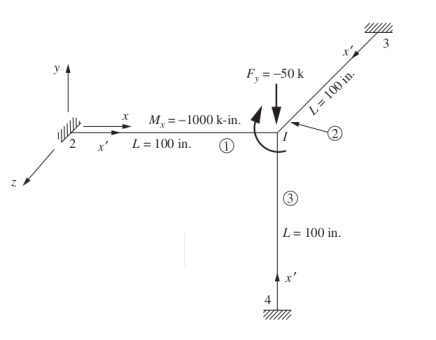
\includegraphics[width=20em]{phy_020_strs_11_06.jpg}

Çözüm

Üç kiriş parçası uzunluk, madde, yapı açısından birbirlerine eşit olduğu için
$k$ matrisini bir kere hesaplamak yeterli. 

\begin{minted}[fontsize=\footnotesize]{python}
from sympy.matrices import Matrix
from sympy import symbols, latex
import pickle, pandas as pd
pd.set_option('display.max_columns', None)
import sys; sys.path.append('../phy_020_strs_08')
import dfutil

A,G,J,E,L,Iy,Iz = symbols("A,G,J,E,L,Iy,Iz")
Mall = pickle.load(open('Mall.pkl','rb'))

D = {E: 30000, G: 10000, J:50, Iy:100, Iz:100, A:10, L:100}
kprime = Mall.subs(D)
print (latex(kprime)[:100], '..')
\end{minted}

\begin{verbatim}
\left[\begin{array}{cccccccccccc}3000 & 0.0 & 0.0 & 0.0 & 0.0 & 0.0 & -3000 & 0.0 & 0.0 & 0.0 & 0.0  ..
\end{verbatim}

$$
{\scriptsize
\left[\begin{array}{cccccccccccc}3000 & 0 & 0 & 0 & 0 & 0 & -3000 & 0 & 0 & 0 & 0 & 0\\0 & 36 & 0 & 0 & 0 & 1800 & 0 & -36 & 0 & 0 & 0 & 1800\\0 & 0 & 36 & 0 & -1800 & 0 & 0 & 0 & -36 & 0 & -1800 & 0\\0 & 0 & 0 & 5000 & 0 & 0 & 0 & 0 & 0 & -5000 & 0 & 0\\0 & 0 & -1800 & 0 & 120000 & 0 & 0 & 0 & 1800 & 0 & 60000 & 0\\0 & 1800 & 0 & 0 & 0 & 120000 & 0 & -1800 & 0 & 0 & 0 & 60000\\-3000 & 0 & 0 & 0 & 0 & 0 & 3000 & 0 & 0 & 0 & 0 & 0\\0 & -36 & 0 & 0 & 0 & -1800 & 0 & 36 & 0 & 0 & 0 & -1800\\0 & 0 & -36 & 0 & 1800 & 0 & 0 & 0 & 36 & 0 & 1800 & 0\\0 & 0 & 0 & -5000 & 0 & 0 & 0 & 0 & 0 & 5000 & 0 & 0\\0 & 0 & -1800 & 0 & 60000 & 0 & 0 & 0 & 1800 & 0 & 120000 & 0\\0 & 1800 & 0 & 0 & 0 & 60000 & 0 & -1800 & 0 & 0 & 0 & 120000\end{array}\right]
}
$$

Geri kalan her parça için dönüş matrislerini hesaplamak.

Parça 1

Önce parça 1 hesapları yapalım, bu parça düğüm 2 noktasından başlayıp
düğüm 1 noktasına gidiyor. O zaman $x'$ ekseni için

$$
l = 1, \quad m = 0, \quad n = 0, \quad D = 1
$$

Diger hesaplar

$$
I_y = -\frac{m_x}{D}, \quad
m_y = \frac{1}{D}, \quad
n_y = 0
$$

$$
i_z = -\frac{l_x n_x}{D} = 0, \quad
m_z = -\frac{m_x n_x}{D} = 0, \quad
n_z = D = 1
$$

Matris içinde gösterirsek,

$$
\lambda = \left[\begin{array}{ccc}
1 & 0 & 0 \\ 0 & 1 & 0 \\ 0 & 0 & 1
\end{array}\right]
$$

Sonuç şaşırtıcı olmasa gerek, çünkü yeni $x$ eski $x$ ile aynı. Bu parça için
sanki eksen hiç değişmesin demiş olduk ve sonuç olarak çarpılınca hiçbir
değişiklik yaratmayacak birim matrisi elde ettik. Bu matrisi büyük $T$ içinde
köşegenlere parça parça yerleştirince yine birim matris elde edilir, yani
$T^T k'T$ aynı $k'$ matrisini verir.

\begin{minted}[fontsize=\footnotesize]{python}
T_P1 = np.eye(12,12)
res1 = np.array(kprime)
vars1 = ['u2','v2','w2','phi2x','phi2y','phi2z','u1','v1','w1','phi1x','phi1y','phi1z']
df1 = pd.DataFrame(res1,columns=vars1)
\end{minted}

Parça 2

Bu parça düğüm 3 noktasıdan düğüm 1 noktasına gidiyor. O zaman $x'$ ekseni
global $z$ ekseni ile aynı şey, o zaman ve yine önceki formüllere bakarak,

$$
\lambda = \left[\begin{array}{ccc}
0 & 0 & 1 \\ 0 & 1 & 0 \\ -1 & 0 & 0
\end{array}\right]
$$

elde ederiz. $T$ matrisi suna benzer,

\begin{minted}[fontsize=\footnotesize]{python}
T_P2 = np.array([
[0, 0,1, 0,0,0, 0,0,0, 0,0,0 ],
[0, 1,0, 0,0,0, 0,0,0, 0,0,0 ],
[-1,0,0, 0,0,0, 0,0,0, 0,0,0],
[0, 0,0, 0,0,1, 0,0,0, 0,0,0 ],
[0, 0,0, 0,1,0, 0,0,0, 0,0,0],
[0, 0,0,-1,0,0, 0,0,0, 0,0,0],
[0, 0,0, 0,0,0, 0,0,1, 0,0,0 ],
[0, 0,0, 0,0,0, 0,1,0, 0,0,0 ],
[0, 0,0, 0,0,0,-1,0,0, 0,0,0],
[0, 0,0, 0,0,0, 0,0,0, 0,0,1],
[0, 0,0, 0,0,0, 0,0,0, 0,1,0 ],
[0, 0,0, 0,0,0, 0,0,0,-1,0,0]])

res2 = T_P2.transpose()*kprime*T_P2
vars2 = ['u3','v3','w3','phi3x','phi3y','phi3z','u1','v1','w1','phi1x','phi1y','phi1z']
df2 = pd.DataFrame(np.array(res2),columns=vars2)
print (latex(res2)[:100],'..')
\end{minted}

\begin{verbatim}
\left[\begin{array}{cccccccccccc}36 & 0 & 0 & 0 & 1800 & 0 & -36 & 0 & 0 & 0 & 1800 & 0\\0 & 36 & 0  ..
\end{verbatim}

$$
\scriptsize
\left[\begin{array}{cccccccccccc}36 & 0 & 0 & 0 & 1800 & 0 & -36 & 0 & 0 & 0 &
    1800 & 0\\0 & 36 & 0 & -1800 & 0 & 0 & 0 & -36 & 0 & -1800 & 0 & 0\\0 & 0 &
    3000 & 0 & 0 & 0 & 0 & 0 & -3000 & 0 & 0 & 0\\0 & -1800 & 0 & 120000 & 0 & 0
    & 0 & 1800 & 0 & 60000 & 0 & 0\\1800 & 0 & 0 & 0 & 120000 & 0 & -1800 & 0 &
    0 & 0 & 60000 & 0\\0 & 0 & 0 & 0 & 0 & 5000 & 0 & 0 & 0 & 0 & 0 & -5000\\-36
    & 0 & 0 & 0 & -1800 & 0 & 36 & 0 & 0 & 0 & -1800 & 0\\0 & -36 & 0 & 1800 & 0
    & 0 & 0 & 36 & 0 & 1800 & 0 & 0\\0 & 0 & -3000 & 0 & 0 & 0 & 0 & 0 & 3000 &
    0 & 0 & 0\\0 & -1800 & 0 & 60000 & 0 & 0 & 0 & 1800 & 0 & 120000 & 0 &
    0\\1800 & 0 & 0 & 0 & 60000 & 0 & -1800 & 0 & 0 & 0 & 120000 & 0\\0 & 0 & 0
    & 0 & 0 & -5000 & 0 & 0 & 0 & 0 & 0 & 5000\end{array}\right]
$$

Parça 3

Bu parça için $x'$ eksenini düğüm 4'ten düğüm 1'e gidiyor şekilde ayarlıyoruz,

$$
l = \frac{0 - 0}{100} = 0, \quad
m = \frac{0 - (-100)}{100} = 1, \quad
n = \frac{0 - 0}{100} = 0
$$

Ayrica $D = 1$.

Simdi $l,m,n$ hesaplanabilir,

$$
l_y = - \frac{m}{D} = -1, \quad
m_y = \frac{L}{D} = 0, \quad
n_y = 0
$$

$$
l_z = - \frac{ln}{D} = 0, \quad
m_z = - \frac{mn}{D} = 0, \quad
n_z = D = 1
$$

O zaman

$$
[ \lambda ] = \left[\begin{array}{rrr}
0 & 1 & 1 \\ -1 & 0 & 0 \\ 0 & 0 & 1
\end{array}\right]
$$

\begin{minted}[fontsize=\footnotesize]{python}
T_P3 = np.array([
[0, 1,0, 0,0,0, 0,0,0, 0, 0,0 ],
[-1,0,0, 0,0,0, 0,0,0, 0, 0,0 ],
[0, 0,1, 0,0,0, 0,0,0, 0, 0,0],
[0, 0,0, 0,1,0, 0,0,0, 0, 0,0 ],
[0, 0,0,-1,0,0, 0,0,0, 0, 0,0],
[0, 0,0, 0,0,1, 0,0,0, 0, 0,0],
[0, 0,0, 0,0,0, 0,1,0, 0, 0,0 ],
[0, 0,0, 0,0,0,-1,0,0, 0, 0,0 ],
[0, 0,0, 0,0,0, 0,0,1, 0, 0,0],
[0, 0,0, 0,0,0, 0,0,0, 0, 1,0],
[0, 0,0, 0,0,0, 0,0,0,-1, 0,0 ],
[0, 0,0, 0,0,0, 0,0,0, 0, 0,1]])

res3 = T_P3.transpose()*kprime*T_P3
vars3 = ['u4','v4','w4','phi4x','phi4y','phi4z','u1','v1','w1','phi1x','phi1y','phi1z']
df3 = pd.DataFrame(np.array(res3),columns=vars3)
print (latex(res3)[:100],'..')
\end{minted}

\begin{verbatim}
\left[\begin{array}{cccccccccccc}36 & 0 & 0 & 0 & 0 & -1800 & -36 & 0 & 0 & 0 & 0 & -1800\\0 & 3000  ..
\end{verbatim}

$$  
\scriptsize
\left[\begin{array}{cccccccccccc}36 & 0 & 0 & 0 & 0 & -1800 & -36 & 0 & 0 & 0 &
    0 & -1800\\0 & 3000 & 0 & 0 & 0 & 0 & 0 & -3000 & 0 & 0 & 0 & 0\\0 & 0 & 36
    & 1800 & 0 & 0 & 0 & 0 & -36 & 1800 & 0 & 0\\0 & 0 & 1800 & 120000 & 0 & 0 &
    0 & 0 & -1800 & 60000 & 0 & 0\\0 & 0 & 0 & 0 & 5000 & 0 & 0 & 0 & 0 & 0 &
    -5000 & 0\\-1800 & 0 & 0 & 0 & 0 & 120000 & 1800 & 0 & 0 & 0 & 0 &
    60000\\-36 & 0 & 0 & 0 & 0 & 1800 & 36 & 0 & 0 & 0 & 0 & 1800\\0 & -3000 & 0
    & 0 & 0 & 0 & 0 & 3000 & 0 & 0 & 0 & 0\\0 & 0 & -36 & -1800 & 0 & 0 & 0 & 0
    & 36 & -1800 & 0 & 0\\0 & 0 & 1800 & 60000 & 0 & 0 & 0 & 0 & -1800 & 120000
    & 0 & 0\\0 & 0 & 0 & 0 & -5000 & 0 & 0 & 0 & 0 & 0 & 5000 & 0\\-1800 & 0 & 0
    & 0 & 0 & 60000 & 1800 & 0 & 0 & 0 & 0 & 120000\end{array}\right]
$$

\begin{minted}[fontsize=\footnotesize]{python}
all_vars = ['u1','v1','w1','phi1x','phi1y','phi1z',\
            'u2','v2','w2','phi2x','phi2y','phi2z',\
            'u3','v3','w3','phi3x','phi3y','phi3z',\
            'u4','v4','w4','phi4x','phi4y','phi4z']
df1f = dfutil.expand_dataframe(df1,all_vars)
df2f = dfutil.expand_dataframe(df2,all_vars)
df3f = dfutil.expand_dataframe(df3,all_vars)
df_super = df1f + df2f + df3f
drop_cols = ['u2','v2','w2','phi2x','phi2y','phi2z', \
             'u3','v3','w3','phi3x','phi3y','phi3z',\
             'u4','v4','w4','phi4x','phi4y','phi4z']
df_super = dfutil.drop_col_row(df_super,drop_cols)
df_super = df_super.applymap(lambda x: np.round(np.float(x),0))
print (df_super)
\end{minted}

\begin{verbatim}
           u1      v1      w1     phi1x     phi1y     phi1z
u1     3072.0     0.0     0.0       0.0   -1800.0    1800.0
v1        0.0  3072.0     0.0    1800.0       0.0   -1800.0
w1        0.0     0.0  3072.0   -1800.0    1800.0       0.0
phi1x     0.0  1800.0 -1800.0  245000.0       0.0       0.0
phi1y -1800.0     0.0  1800.0       0.0  245000.0       0.0
phi1z  1800.0 -1800.0     0.0       0.0       0.0  245000.0
\end{verbatim}


\begin{minted}[fontsize=\footnotesize]{python}
import numpy.linalg as lin
d = lin.solve(df_super,np.array([[0,-50,0,-1000,0,0]]).T)
d = pd.DataFrame(d,index=df_super.index)
d
\end{minted}

\begin{verbatim}
Out[1]: 
              0
u1     0.000071
v1    -0.013995
w1    -0.002352
phi1x -0.003996
phi1y  0.000018
phi1z -0.000103
\end{verbatim}

Parca 1

\begin{minted}[fontsize=\footnotesize]{python}
d_expanded1 = pd.DataFrame(d,index=vars1).fillna(0)
f1 = np.dot(np.dot(kprime, T_P1), d_expanded1)
f1
\end{minted}

\begin{verbatim}
Out[1]: 
array([[-0.212947726538524],
       [0.317807629532996],
       [0.0526267712100185],
       [19.9804522034949],
       [-3.16535930819590],
       [18.9906685952123],
       [0.212947726538524],
       [-0.317807629532996],
       [-0.0526267712100185],
       [-19.9804522034949],
       [-2.09731781280595],
       [12.7900943580873]], dtype=object)
\end{verbatim}

Parca 2

\begin{minted}[fontsize=\footnotesize]{python}
d_expanded2 = pd.DataFrame(d,index=vars2).fillna(0)
f2 = np.dot(np.dot(kprime, T_P2), d_expanded2)
f2
\end{minted}

\begin{verbatim}
Out[1]: 
array([[7.05566800597642],
       [7.69678764990490],
       [-0.0294858721432362],
       [0.516714519760416],
       [0.940272859466836],
       [264.956669274276],
       [-7.05566800597642],
       [-7.69678764990490],
       [0.0294858721432362],
       [-0.516714519760416],
       [2.00831435485679],
       [504.722095716214]], dtype=object)
\end{verbatim}

Parca 2

\begin{minted}[fontsize=\footnotesize]{python}
d_expanded3 = pd.DataFrame(d,index=vars3).fillna(0)
f3 = np.dot(np.dot(kprime, T_P3), d_expanded3)
f3
\end{minted}

\begin{verbatim}
Out[1]: 
array([[41.9854047205621],
       [-0.183461854395287],
       [-7.10829477718644],
       [-0.0890034579491625],
       [235.532025638353],
       [-6.07280560120188],
       [-41.9854047205621],
       [0.183461854395287],
       [7.10829477718644],
       [0.0890034579491625],
       [475.297452080291],
       [-12.2733798383269]], dtype=object)
\end{verbatim}








[devam edecek]

Kaynaklar

[1] Bayramlı, {\em Fizik, Materyel Mekaniği 7}

[2] Logan, {\em A First Course in the Finite Element Method, 6th Ed}

[3] Witt {\em Concepts and Apps of FEM}

[4] Bayramlı, {\em Fizik, Materyel Mekaniği 9}

[5] Dunn, {\em 3D Math Primer for Graphics and Game Development}

[6] Stasa, {\em Applied Finite Element Analysis for Engineers}

\end{document}

